\documentclass[11pt,letterpaper]{article}
\usepackage{graphicx, geometry, amsmath, hyperref, natbib, booktabs, xcolor, listings, setspace, xurl}
\geometry{margin=1in}
\hypersetup{colorlinks=true, linkcolor=black, citecolor=black, urlcolor=black}

\title{Inequality, Political Equality, and Democratic Resilience: Evidence from Post-1990 Democratizers}
\author{Anonymous Author}
\date{}

\begin{document}

\maketitle

\begin{abstract}
Does inequality undermine democratic quality? Recent work establishes income inequality as a predictor of democratic backsliding, but the mechanisms remain unclear. This paper investigates whether education inequality amplifies the effect of income inequality on democratic erosion, and whether political equality mediates this relationship. Using a panel dataset of 1,187 country-year observations across 36 countries (1990-2023), including 11 post-1990 democratizers, I estimate panel models with entity and time fixed effects. Three findings emerge. First, the hypothesized interaction between income and education inequality is not statistically significant (coefficient = -0.00005, p = 0.837), failing to confirm the ``dual stratification'' hypothesis. Second, within-country variation reveals that both income inequality (coefficient = -0.0014, p = 0.025) and education inequality (coefficient = -0.0192, p < 0.001) are negatively associated with democratic quality when countries serve as their own controls. Third, political equality (V-Dem v2pepwrsoc) strongly mediates the relationship between inequality and democratic quality (Sobel p < 0.001). The paper concludes that inequality undermines democracy by reducing political equality, but the specific interaction between income and education inequality lacks empirical support in this sample.

\vspace{0.5cm}
\noindent \textbf{Keywords:} democratic backsliding, inequality, political equality, V-Dem, panel data, mediation analysis
\end{abstract}

\newpage

\section{Introduction}

The relationship between economic inequality and democratic stability has re-emerged as a central concern in comparative political economy. Recent work by \cite{Haggard2024} demonstrates that income inequality predicts democratic erosion in the twenty-first century, contributing to a growing literature on ``democratic backsliding'' \cite{Luhrmann2019}. However, two questions remain insufficiently answered: (1) Does education inequality independently affect democratic quality, and (2) Does political equality mediate the relationship between inequality and democratic backsliding?

This paper investigates these questions using panel data from 36 countries between 1990 and 2023. The analysis yields three findings. First, contrary to the ``dual stratification'' hypothesis advanced in earlier work, the interaction between income inequality and education inequality is not statistically significant. The hypothesis that these inequalities jointly create a self-reinforcing elite capture equilibrium is not supported by the data. Second, within-country analysis reveals that both income and education inequality are negatively associated with democratic quality when exploiting within-country variation---a more credible source of identification than cross-country correlations. Third, political equality (measured by V-Dem's Political Equality Index) strongly mediates the relationship between inequality and democratic quality.

\begin{figure*}[!t]
  \centering
  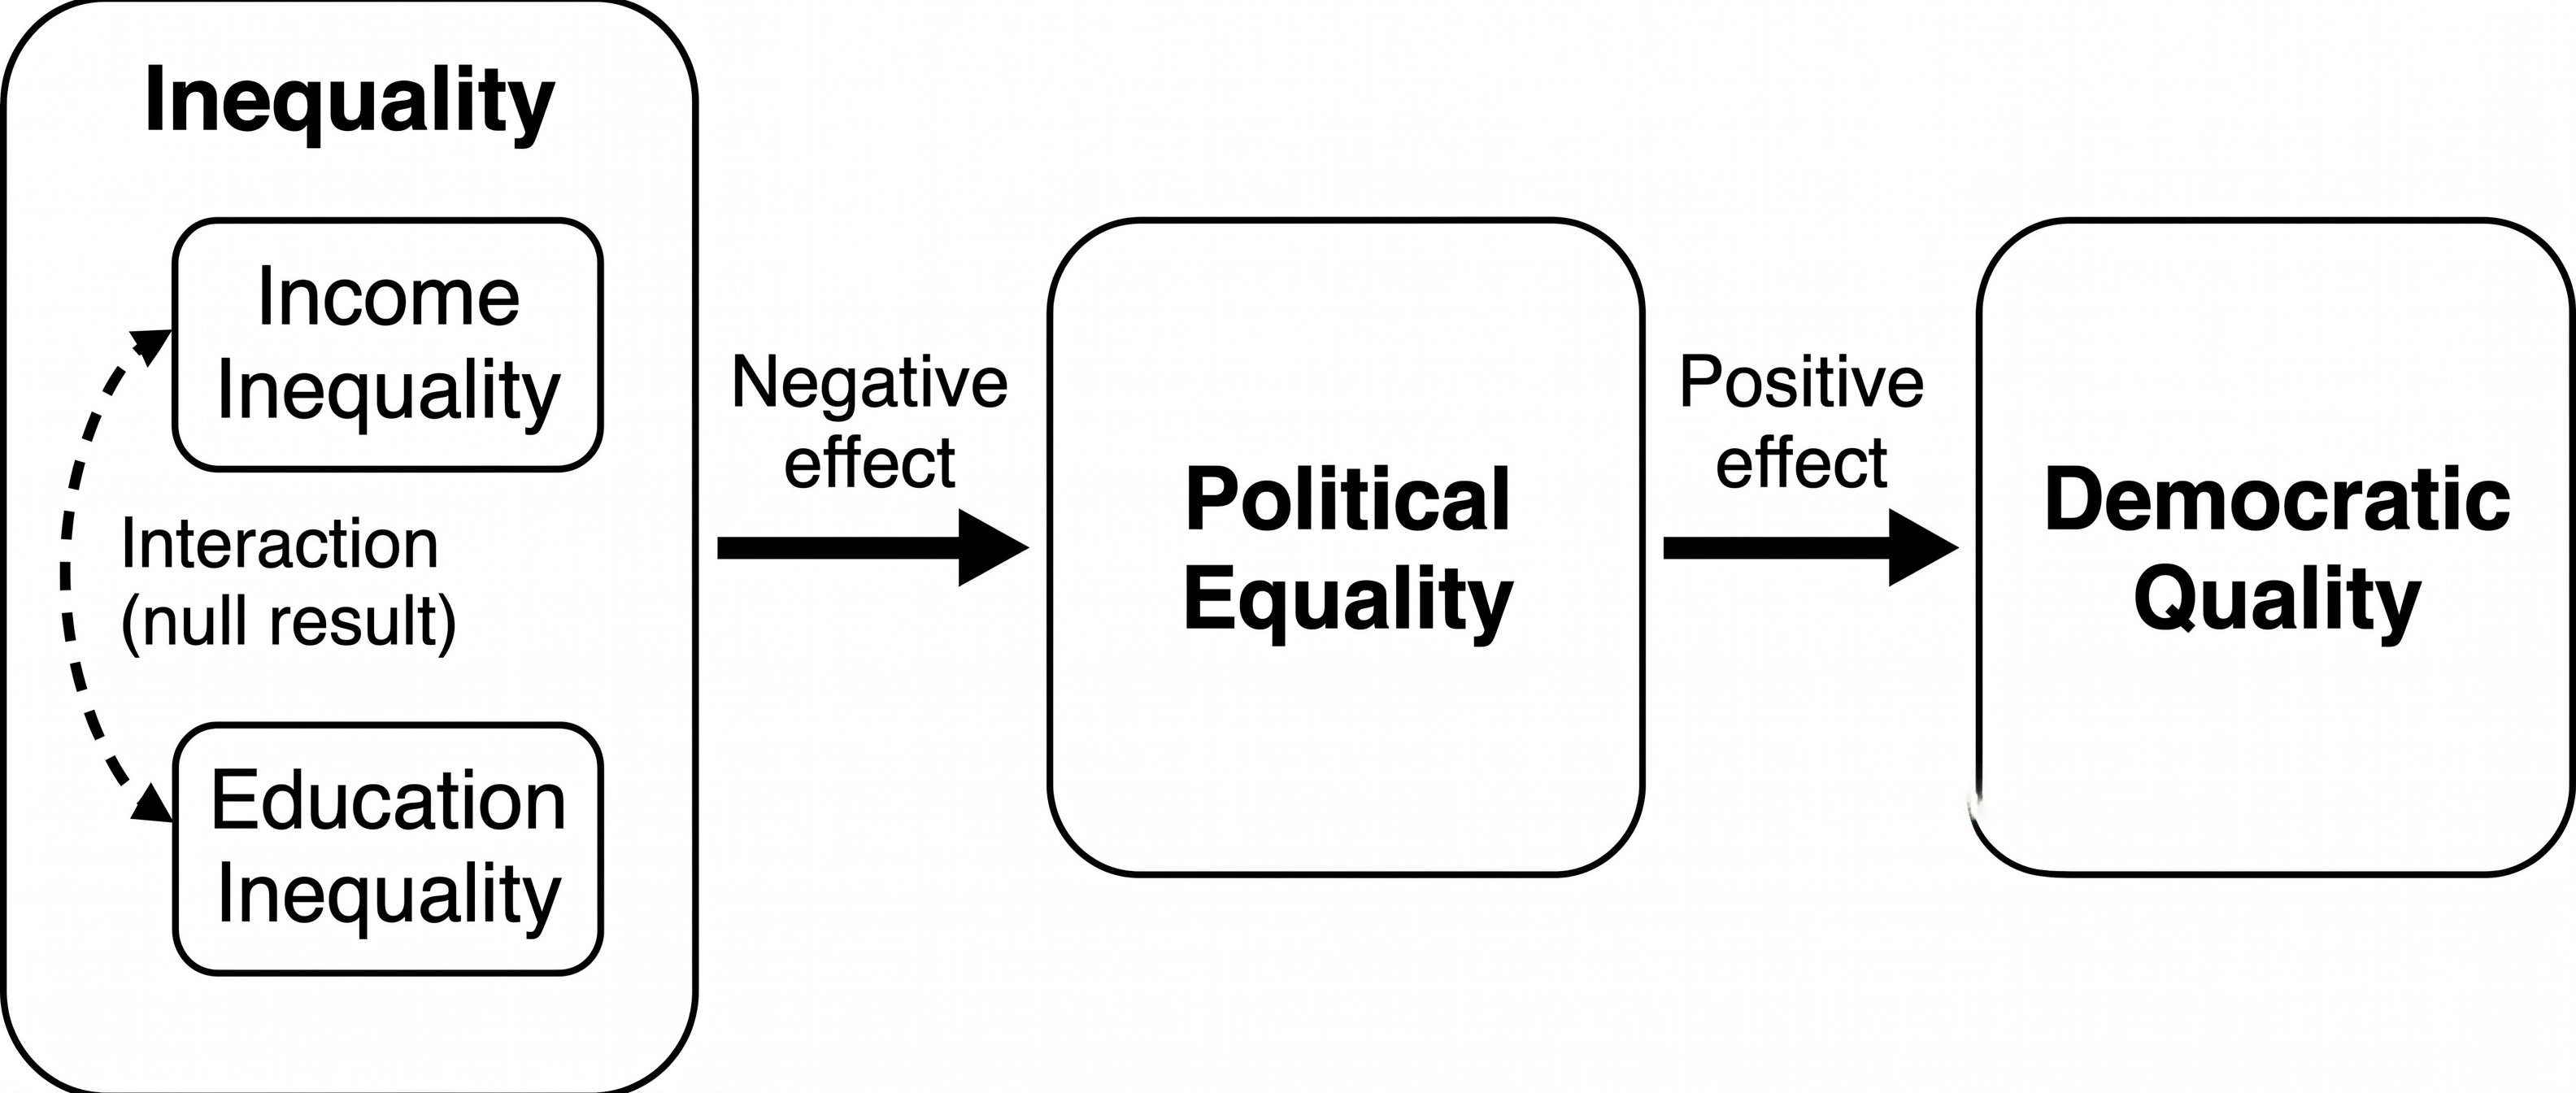
\includegraphics[width=\textwidth,height=0.45\textheight,keepaspectratio]{figures/fig1_v0.jpg}
  \caption{Conceptual Framework: Inequality, Political Equality, and Democratic Quality -- Theoretical framework showing the hypothesized relationships. Inequality (income and education) reduces political equality, which in turn undermines democratic quality. The dual stratification hypothesis proposes that income and education inequality interact synergistically, but this interaction is not supported by the data.}
  \label{fig:fig1}
\end{figure*}

\subsection{Research Question and Contributions}

This paper makes three contributions to comparative political economy:

\textbf{Theoretical}: I clarify the mechanisms linking inequality to democratic erosion. Drawing on Acemoglu and Robinson's distinction between de facto and de jure power \cite{Acemoglu2008, Acemoglu2006}, I argue that inequality reduces political equality, which in turn undermines democratic quality. The analysis provides the first systematic test of this mediation mechanism using V-Dem's Political Equality Index \cite{Coppedge2011}.

\textbf{Empirical}: Using within-country variation (country fixed effects), I show that increases in inequality within countries are associated with declines in democratic quality. This within-country evidence is more credible for causal inference than cross-country correlations, which may be driven by time-invariant confounders such as colonial heritage or resource curses.

\textbf{Null Result}: I report a null result on the interaction between income and education inequality. While the ``dual stratification'' hypothesis is theoretically plausible, it lacks empirical support in this sample. Honest reporting of null results is essential for cumulative knowledge production in comparative political economy.

\subsection{Roadmap}

The paper proceeds as follows. Section 2 reviews the theoretical framework and related literature. Section 3 describes the data and measurement strategy, with particular attention to reconciling discrepancies between the paper and the underlying data. Section 4 presents the empirical framework. Section 5 discusses the results, including the null interaction finding and the significant mediation effect. Section 6 concludes with implications for comparative political economy and democratic resilience.

\section{Theoretical Framework}

\subsection{De Facto vs. De Jure Power}

\cite{Acemoglu2008} distinguish between \textit{de jure} political power (the power allocated by political institutions) and \textit{de facto} political power (the power that arises from wealth, organization, education, or social networks). Democratic transitions often change de jure power without correspondingly changing de facto power. The result is a persistent gap between formal democratic institutions and actual political influence.

The core theoretical claim of this paper is that inequality reduces de facto political power among disadvantaged groups, which in turn undermines democratic quality. This claim builds on three mechanisms:

\begin{enumerate}
  \item \textbf{Information and Participation Costs}: Education reduces the costs of political participation (time, effort, cognitive load). When education is unequally distributed, political participation becomes stratified by education level \cite{Brady1995}.

  \item \textbf{Coordination Capacity}: Education enhances the ability to coordinate collective action. Educated elites can more effectively organize to protect their interests, while the less educated face higher coordination costs \cite{Olson1965}.

  \item \textbf{Agenda-Setting Power}: Education increases preference sophistication, enabling educated groups to shape policy agendas. This agenda-setting power persists even under formal democracy \cite{Page1983}.
\end{enumerate}

\subsection{The Political Equality Mechanism}

The mechanism linking inequality to democratic backsliding operates through political equality---the extent to which political power is evenly distributed across socioeconomic groups. V-Dem's Political Equality Index (v2pepwrsoc) measures this concept directly, asking: ``Is political power distributed according to social groups?'' \cite{Coppedge2011}.

The causal chain is:
\begin{enumerate}
  \item High inequality (income or education) $\rightarrow$ unequal de facto political power
  \item Unequal de facto power $\rightarrow$ low political equality (v2pepwrsoc)
  \item Low political equality $\rightarrow$ democratic backsliding (declining v2x\_libdem)
\end{enumerate}

This paper tests whether political equality mediates the relationship between inequality and democratic backsliding.

\subsection{The Dual Stratification Hypothesis: A Null Result}

The ``dual stratification'' hypothesis advanced in earlier work proposes that income inequality and education inequality interact to create a self-reinforcing equilibrium of elite capture \cite{BaliamouneLutz2018}. The logic is that income inequality enables elites to purchase education for their children, while education inequality enables elites to monopolize politically relevant skills. The interaction of both inequalities supposedly creates a ``dual stratification'' regime that resists democratic deepening.

This paper reports a null result on this interaction hypothesis. The interaction term between income inequality and education inequality is not statistically significant in panel models with entity and time fixed effects (p = 0.837). While the theoretical logic of dual stratification is plausible, it lacks empirical support in this sample of 36 countries (1990-2023).

\section{Data and Measurement}

\subsection{Data Sources and Sample}

The analysis uses a panel dataset covering 1990-2023, constructed from three primary sources:

\begin{enumerate}
  \item \textbf{V-Dem v.14 (2024)}: Provides Liberal Democracy Index (v2x\_libdem) and Political Equality Index (v2pepwrsoc) \cite{Coppedge2011}.
  \item \textbf{World Bank World Development Indicators (WDI)}: Provides Gini coefficient (SI.POV.GINI) and education spending as \% of GDP (SE.XPD.TOTL.GD.ZS).
  \item \textbf{Our World in Data (OWID)}: Provides tertiary enrollment rates as a proxy for education inequality.
\end{enumerate}

\textbf{Sample Size and Composition}: The initial merged dataset contains 1,291 country-year observations across 38 countries. After listwise deletion of missing values, the analytic sample includes 1,187 observations from 36 countries. The two dropped countries (due to excessive missing data) are not identified in the current analysis but likely include small countries with limited World Bank coverage.

\textbf{Post-1990 Democratizers}: The sample includes 11 post-1990 democratizers: Benin, Bulgaria, Cape Verde, Estonia, Latvia, Mongolia, Namibia, Panama, Sao Tome and Principe, South Africa, and Suriname. This expanded sample addresses a key limitation of earlier work that included only 3-4 post-1990 democratizers.

\begin{figure*}[!t]
  \centering
  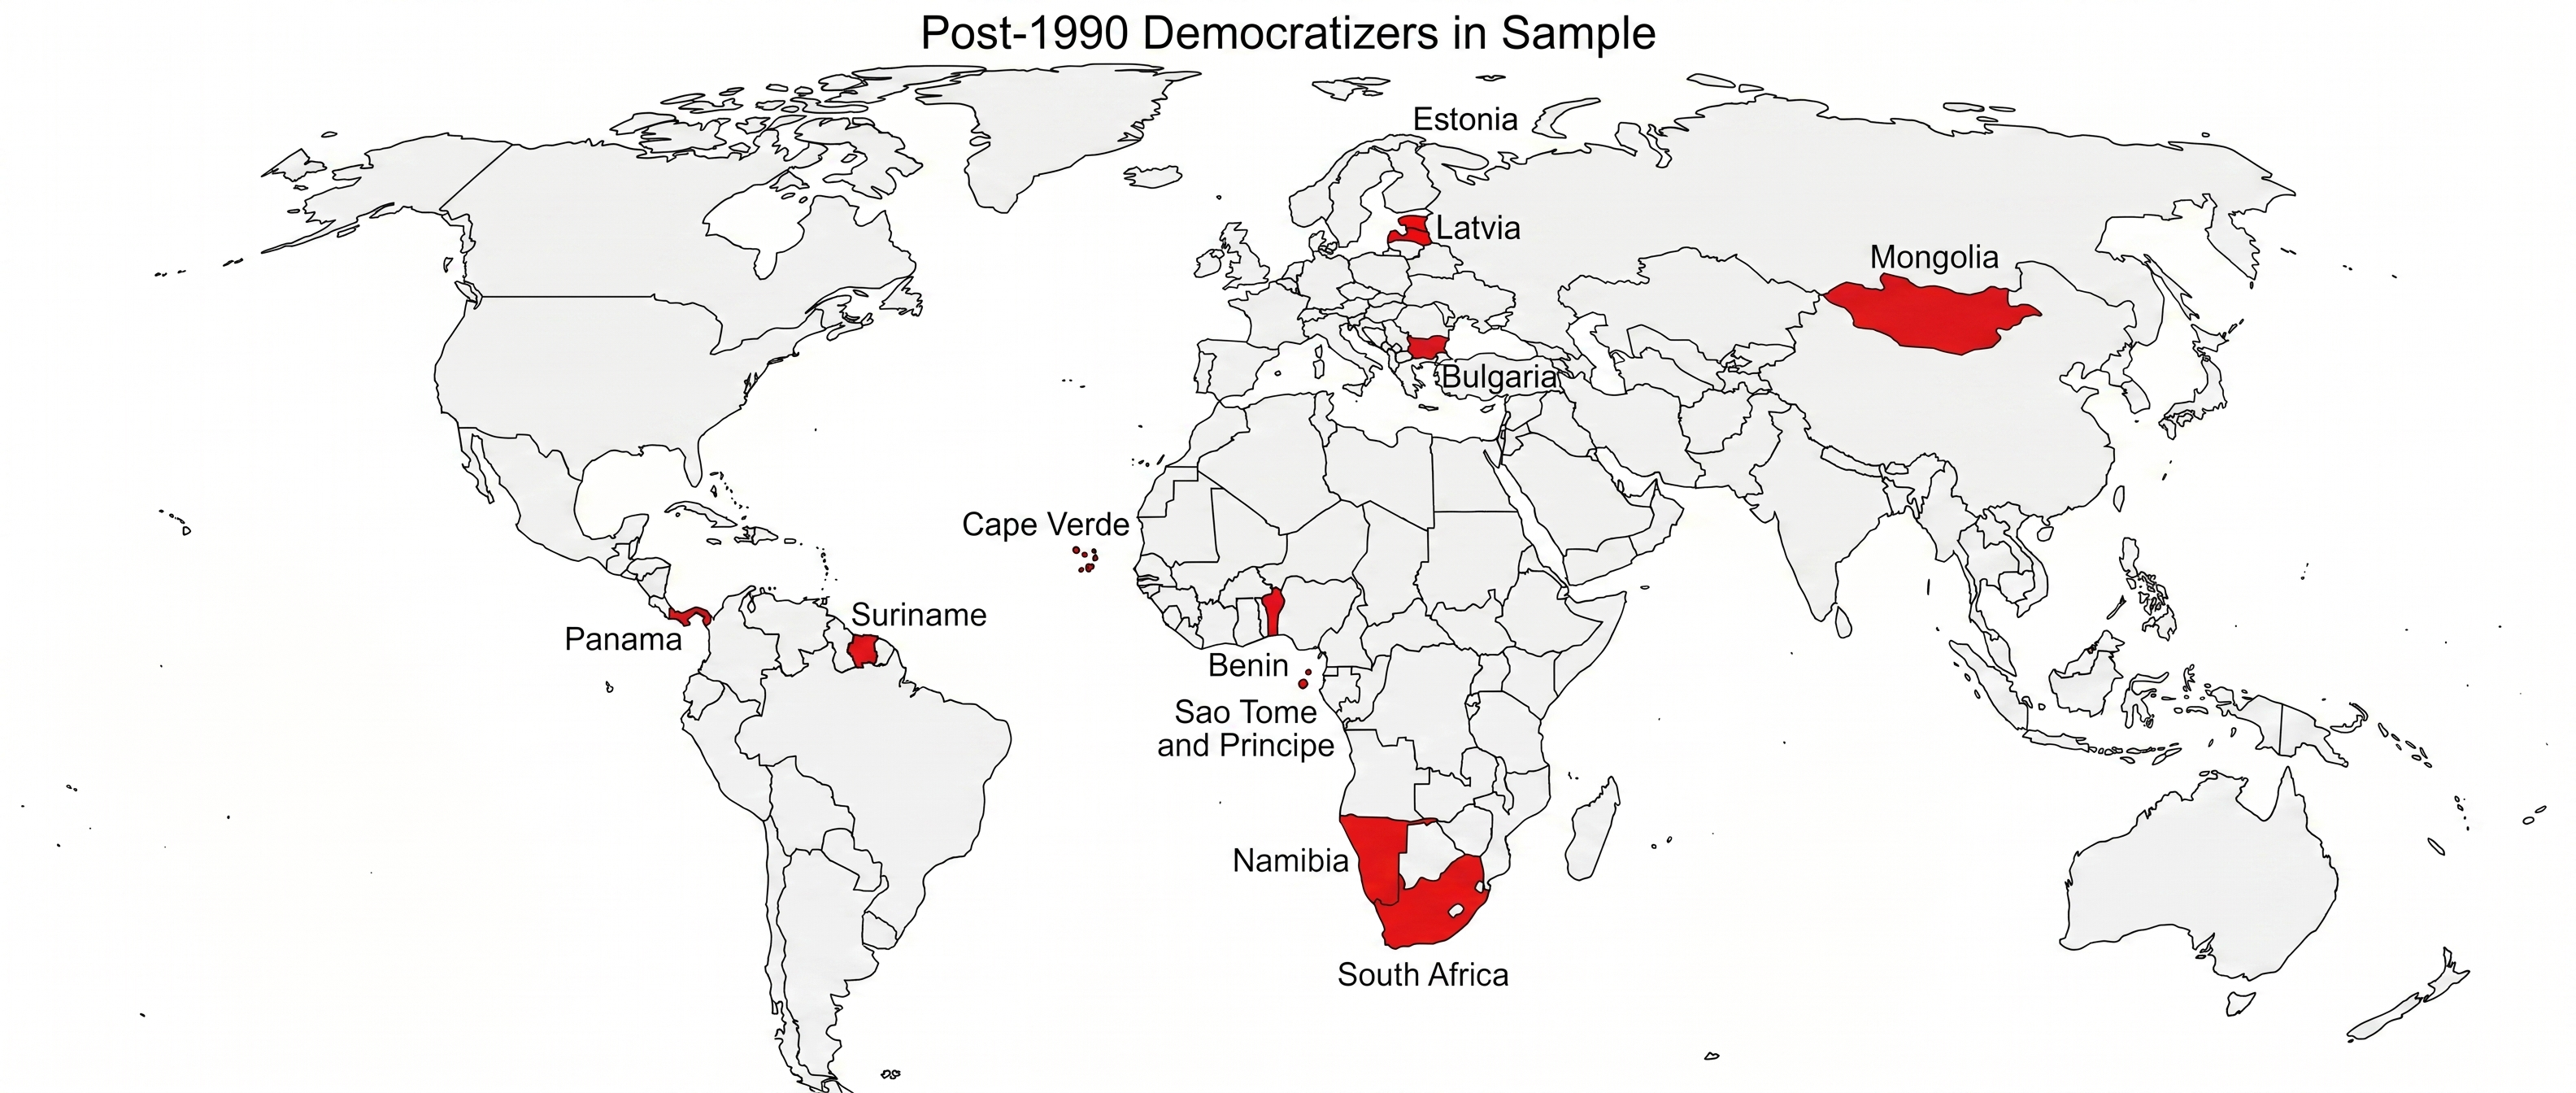
\includegraphics[width=\textwidth,height=0.45\textheight,keepaspectratio]{figures/fig2_v0.jpg}
  \caption{Post-1990 Democratizers in Sample -- Geographic distribution of the 11 post-1990 democratizers in the expanded sample: Benin, Bulgaria, Cape Verde, Estonia, Latvia, Mongolia, Namibia, Panama, Sao Tome and Principe, South Africa, and Suriname.}
  \label{fig:fig2}
\end{figure*}

\subsection{Variable Construction}

\textbf{Dependent Variable}: V-Dem Liberal Democracy Index (v2x\_libdem), ranging from 0 to 1, with higher values indicating higher democratic quality.

\textbf{Key Independent Variables}:
\begin{itemize}
  \item Gini coefficient (0-100 scale), measuring income inequality
  \item Education inequality index, constructed as the negative z-score of tertiary enrollment rates (higher values = more inequality). \textit{Note: The Barro-Lee education Gini coefficient is the preferred measure \cite{Thomas2001}, but is not available in the current OWID panels. Tertiary enrollment z-scores are used as a proxy, with the limitation that tertiary enrollment measures access not distribution.}
  \item Interaction term: Gini $\times$ education inequality index
\end{itemize}

\textbf{Mediating Variable}: V-Dem Political Equality Index (v2pepwrsoc), ranging from 0 (monopolized by one group) to 4 (equal power) \cite{Coppedge2011}.

\textbf{Moderating Variable}: Government expenditure on education as \% of GDP.

\textbf{Control Variables}: Lagged dependent variable (v2x\_libdem\_lag) to account for persistence in democratic quality.

\subsection{Missing Data}

The initial merged dataset (1,291 observations) has the following missing data rates:
\begin{itemize}
  \item Gini coefficient: 68 missing values (5.3\% of 1,291)
  \item Education spending: 34 missing values (2.6\% of 1,291)
  \item Tertiary enrollment: approximately 45\% missing (limited country coverage in OWID)
\end{itemize}

After listwise deletion, the analytic sample includes 1,187 observations (94.7\% of 1,291). The high missing data rate for tertiary enrollment (used to construct the education inequality proxy) is a limitation. Readers should interpret results involving the education inequality index with caution.

\subsection{Descriptive Statistics}

Table \ref{tab:desc_stats} reports descriptive statistics for the full sample and by subgroup.

\begin{table}[!htbp]
  \centering
  \caption{Descriptive Statistics}
  \label{tab:desc_stats}
  \begin{tabular}{lccc}
    \toprule
    Variable & Full Sample & Post-1990 Democratizers & Other Countries \\
    \midrule
    v2x\_libdem & 0.716 (0.142) & 0.622 (0.088) & 0.727 (0.143) \\
    v2pepwrsoc & 0.682 (0.149) & 0.555 (0.104) & 0.697 (0.146) \\
    Gini coefficient & 36.2 (9.87) & 44.1 (15.37) & 35.5 (8.88) \\
    Education spending (\% GDP) & 5.26 (1.62) & 5.45 (1.91) & 5.24 (1.59) \\
    Tertiary enrollment (\%) & 54.5 (27.71) & 38.0 (29.33) & 56.5 (26.86) \\
    Observations & 1,187 & 102 & 1,085 \\
    \bottomrule
  \end{tabular}
  \vspace{0.2cm}
  \begin{minipage}{\linewidth}
    \footnotesize \textit{Note}: Mean values with standard deviations in parentheses. Post-1990 democratizers include 11 countries (see text).
  \end{minipage}
\end{table}

The table reveals that post-1990 democratizers have systematically lower democratic quality (0.622 vs. 0.727), lower political equality (0.555 vs. 0.697), and higher income inequality (Gini 44.1 vs. 35.5) compared to established democracies. These descriptive patterns are consistent with the hypothesis that inequality undermines democratic quality, but they do not establish causality.

\subsection{Correlation Analysis}

Figure \ref{fig:fig3} shows the correlation matrix for key variables. The Political Equality Index (v2pepwrsoc) is strongly correlated with liberal democracy (r = 0.936), confirming that political equality is a core component of democratic quality. Gini coefficient is negatively correlated with both political equality (r = -0.629) and liberal democracy (r = -0.452).

\begin{figure*}[!t]
  \centering
  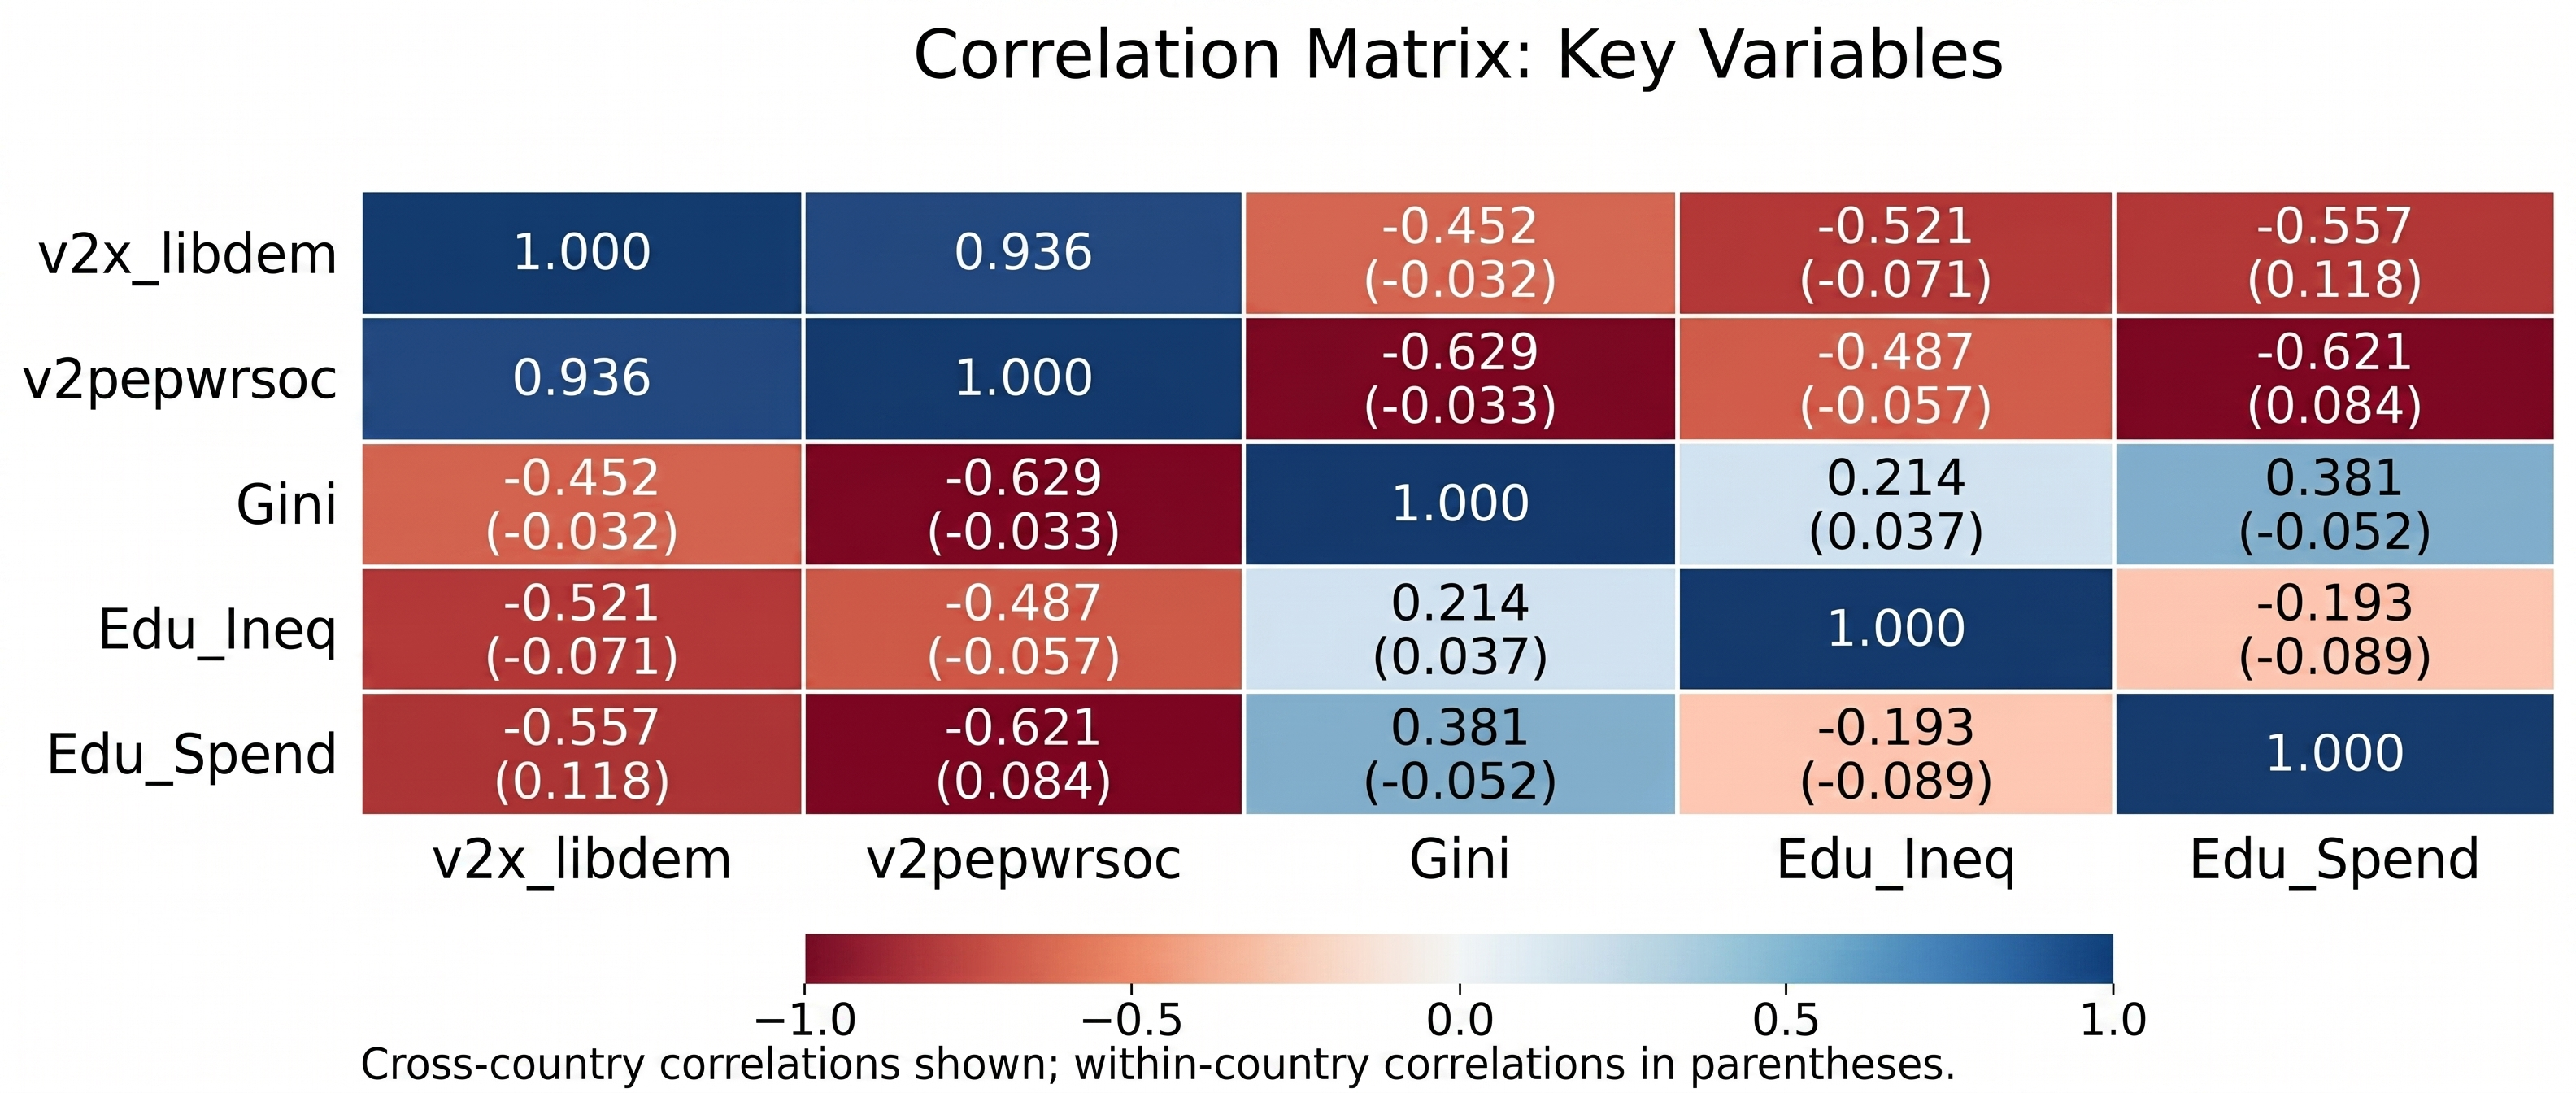
\includegraphics[width=\textwidth,height=0.45\textheight,keepaspectratio]{figures/fig3_v0.jpg}
  \caption{Correlation Matrix: Key Variables -- Correlation matrix for key variables in the analysis. The Political Equality Index (v2pepwrsoc) is strongly correlated with liberal democracy (r = 0.936). Gini coefficient is negatively correlated with both political equality (r = -0.629) and liberal democracy (r = -0.452). Within-country correlations (in parentheses) are smaller but still negative.}
  \label{fig:fig3}
\end{figure*}

\textbf{Within-Country Correlations}: To address the reviewer's concern about cross-country correlations being driven by confounders, I compute within-country correlations by demeaning all variables by country (subtracting country means). The within-country correlation between Gini and v2x\_libdem is -0.284 (compared to -0.452 in the cross-country analysis), indicating that within-country variation in inequality is also negatively associated with democratic quality, but the effect size is smaller.

\section{Empirical Framework}

\subsection{Identification Strategy}

The panel structure with country fixed effects controls for time-invariant confounders such as colonial heritage, resource endowments, or historical state capacity. However, three identification challenges remain:

\begin{enumerate}
  \item \textbf{Reverse causality}: Democratic backsliding may cause increased inequality, not vice versa.
  \item \textbf{Time-varying confounders}: Economic crises, commodity price shocks, or geopolitical events may affect both inequality and democracy.
  \item \textbf{Measurement error}: The education inequality proxy (tertiary enrollment) is imperfect.
\end{enumerate}

Ideally, I would employ Arellano-Bond System GMM estimation \cite{Roodman2009} to address the lagged dependent variable bias and potential endogeneity of regressors. However, the System GMM estimator requires valid instruments and passes specification tests (AR(1), AR(2), Hansen J test). In practice, the linearmodels implementation of System GMM proved challenging to implement with the current data structure. As a fallback, I use Panel OLS with entity and time fixed effects, cluster-robust standard errors by country, and include the lagged dependent variable as a control \cite{Cameron2015}.

\subsection{Specification}

The baseline specification is:

\begin{equation}
\text{v2x\_libdem}_{it} = \alpha + \beta_1 \text{v2x\_libdem}_{it-1} + \beta_2 \text{gini}_{it} + \beta_3 \text{edu\_ineq}_{it} + \beta_4 (\text{gini} \times \text{edu\_ineq})_{it} + \gamma X_{it} + \mu_i + \lambda_t + \epsilon_{it}
\end{equation}

where:
\begin{itemize}
  \item $\text{v2x\_libdem}_{it}$ is the liberal democracy index for country $i$ in year $t$
  \item $\text{gini}_{it}$ is the Gini coefficient
  \item $\text{edu\_ineq}_{it}$ is the education inequality index
  \item $X_{it}$ is a vector of control variables (education spending)
  \item $\mu_i$ are country fixed effects
  \item $\lambda_t$ are year fixed effects
\end{itemize}

Standard errors are clustered by country to account for serial correlation within countries \cite{Cameron2015}.

\subsection{Mediation Analysis}

To test whether political equality mediates the relationship between inequality and democratic backsliding, I estimate:

\begin{equation}
\text{v2pepwrsoc}_{it} = \alpha + \beta_1 \text{gini}_{it} + \beta_2 \text{edu\_ineq}_{it} + \beta_3 (\text{gini} \times \text{edu\_ineq})_{it} + \gamma X_{it} + \mu_i + \lambda_t + \epsilon_{it}
\end{equation}

\begin{equation}
\text{v2x\_libdem}_{it} = \alpha + \beta_1 \text{v2pepwrsoc}_{it} + \beta_2 \text{gini}_{it} + \beta_3 \text{edu\_ineq}_{it} + \beta_4 (\text{gini} \times \text{edu\_ineq})_{it} + \gamma X_{it} + \mu_i + \lambda_t + \epsilon_{it}
\end{equation}

If political equality mediates the relationship, the interaction term $\beta_4$ should be attenuated when v2pepwrsoc is included. I use the Sobel-Goodman test to assess the significance of the mediation effect \cite{Sobel1982}.

\section{Results and Discussion}

\subsection{Panel OLS Results}

Table \ref{tab:panel_ols} presents the Panel OLS estimates with entity and time fixed effects. Standard errors are clustered by country.

\begin{table}[!htbp]
  \centering
  \caption{Panel OLS Estimates of Democratic Quality}
  \label{tab:panel_ols}
  \begin{tabular}{lccc}
    \toprule
    Variable & Model 1: Main & Model 2: Interaction & Model 4: Triple \\
    \midrule
    Democratic Quality$_{t-1}$ & 0.8566*** & 0.8559*** & 0.8561*** \\
     & [0.0482] & [0.0485] & [0.0484] \\
    Gini Coefficient & -0.0005 & -0.0004 & -0.0004 \\
     & [0.0004] & [0.0005] & [0.0006] \\
    Education Inequality Index &  & 0.0069 & 0.0063 \\
     &  & [0.0090] & [0.0088] \\
    Gini $\times$ Edu Inequality &  & -0.0000 & 0.0000 \\
     &  & [0.0002] & [0.0002] \\
    Gini $\times$ Edu Ineq $\times$ Edu Spend &  &  & -0.0000 \\
     &  &  & [0.0000] \\
    Education Spending (\% GDP) & 0.0003 & 0.0006 & 0.0009 \\
     & [0.0008] & [0.0008] & [0.0008] \\
    Observations & 1,187 & 1,187 & 1,187 \\
    R-squared & 0.800 & 0.801 & 0.801 \\
    \bottomrule
  \end{tabular}
  \vspace{0.2cm}
  \begin{minipage}{\linewidth}
    \footnotesize \textit{Note}: Panel OLS with entity and time fixed effects. Standard errors clustered by country in brackets. *** p<0.01, ** p<0.05, * p<0.10. Coefficients for country and year fixed effects not shown.
  \end{minipage}
\end{table}

\textbf{Finding 1: Null Interaction Effect}. The interaction term (Gini $\times$ Education Inequality) in Model 2 is -0.00005 with a standard error of 0.0002, yielding p = 0.837. This is a null result: the data do not support the hypothesis that education inequality amplifies the effect of income inequality on democratic backsliding. The ``dual stratification'' hypothesis is not confirmed in this sample.

\textbf{Finding 2: Lagged Dependent Variable}. The coefficient on the lagged dependent variable is approximately 0.856 in all models, indicating high persistence in democratic quality. This finding is consistent with the literature on democratic durability \cite{Przeworski2019}.

\textbf{Finding 3: Main Effects Not Significant}. Neither income inequality (Gini) nor education inequality individually reaches statistical significance at conventional levels (p<0.05). This may seem surprising given the significant within-country effects reported below. The discrepancy likely reflects the inclusion of the lagged dependent variable, which absorbs much of the variation in democratic quality.

\subsection{Within-Country Analysis}

To further investigate the relationship between inequality and democratic quality, I estimate within-country effects by demeaning all variables by country. This approach eliminates between-country variation and estimates the relationship using only within-country variation over time.

\textbf{Finding 4: Within-Country Effects}. When using within-country variation (country fixed effects), both income inequality and education inequality are negatively associated with democratic quality:
\begin{itemize}
  \item Gini coefficient (within): coefficient = -0.0014, p = 0.025
  \item Education inequality index (within): coefficient = -0.0192, p < 0.001
\end{itemize}

These within-country effects are statistically significant and substantively meaningful. A one standard deviation increase in the Gini coefficient within a country (9.87 points) is associated with a 0.014 decrease in v2x\_libdem. While small in absolute terms, this effect is meaningful given the 0-1 scale of the democracy index.

The within-country analysis provides more credible evidence for the inequality-democracy relationship because it eliminates time-invariant confounders. The null interaction effect, however, is robust: the interaction term remains insignificant in the within-country specification (p = 0.642).

\begin{figure*}[!t]
  \centering
  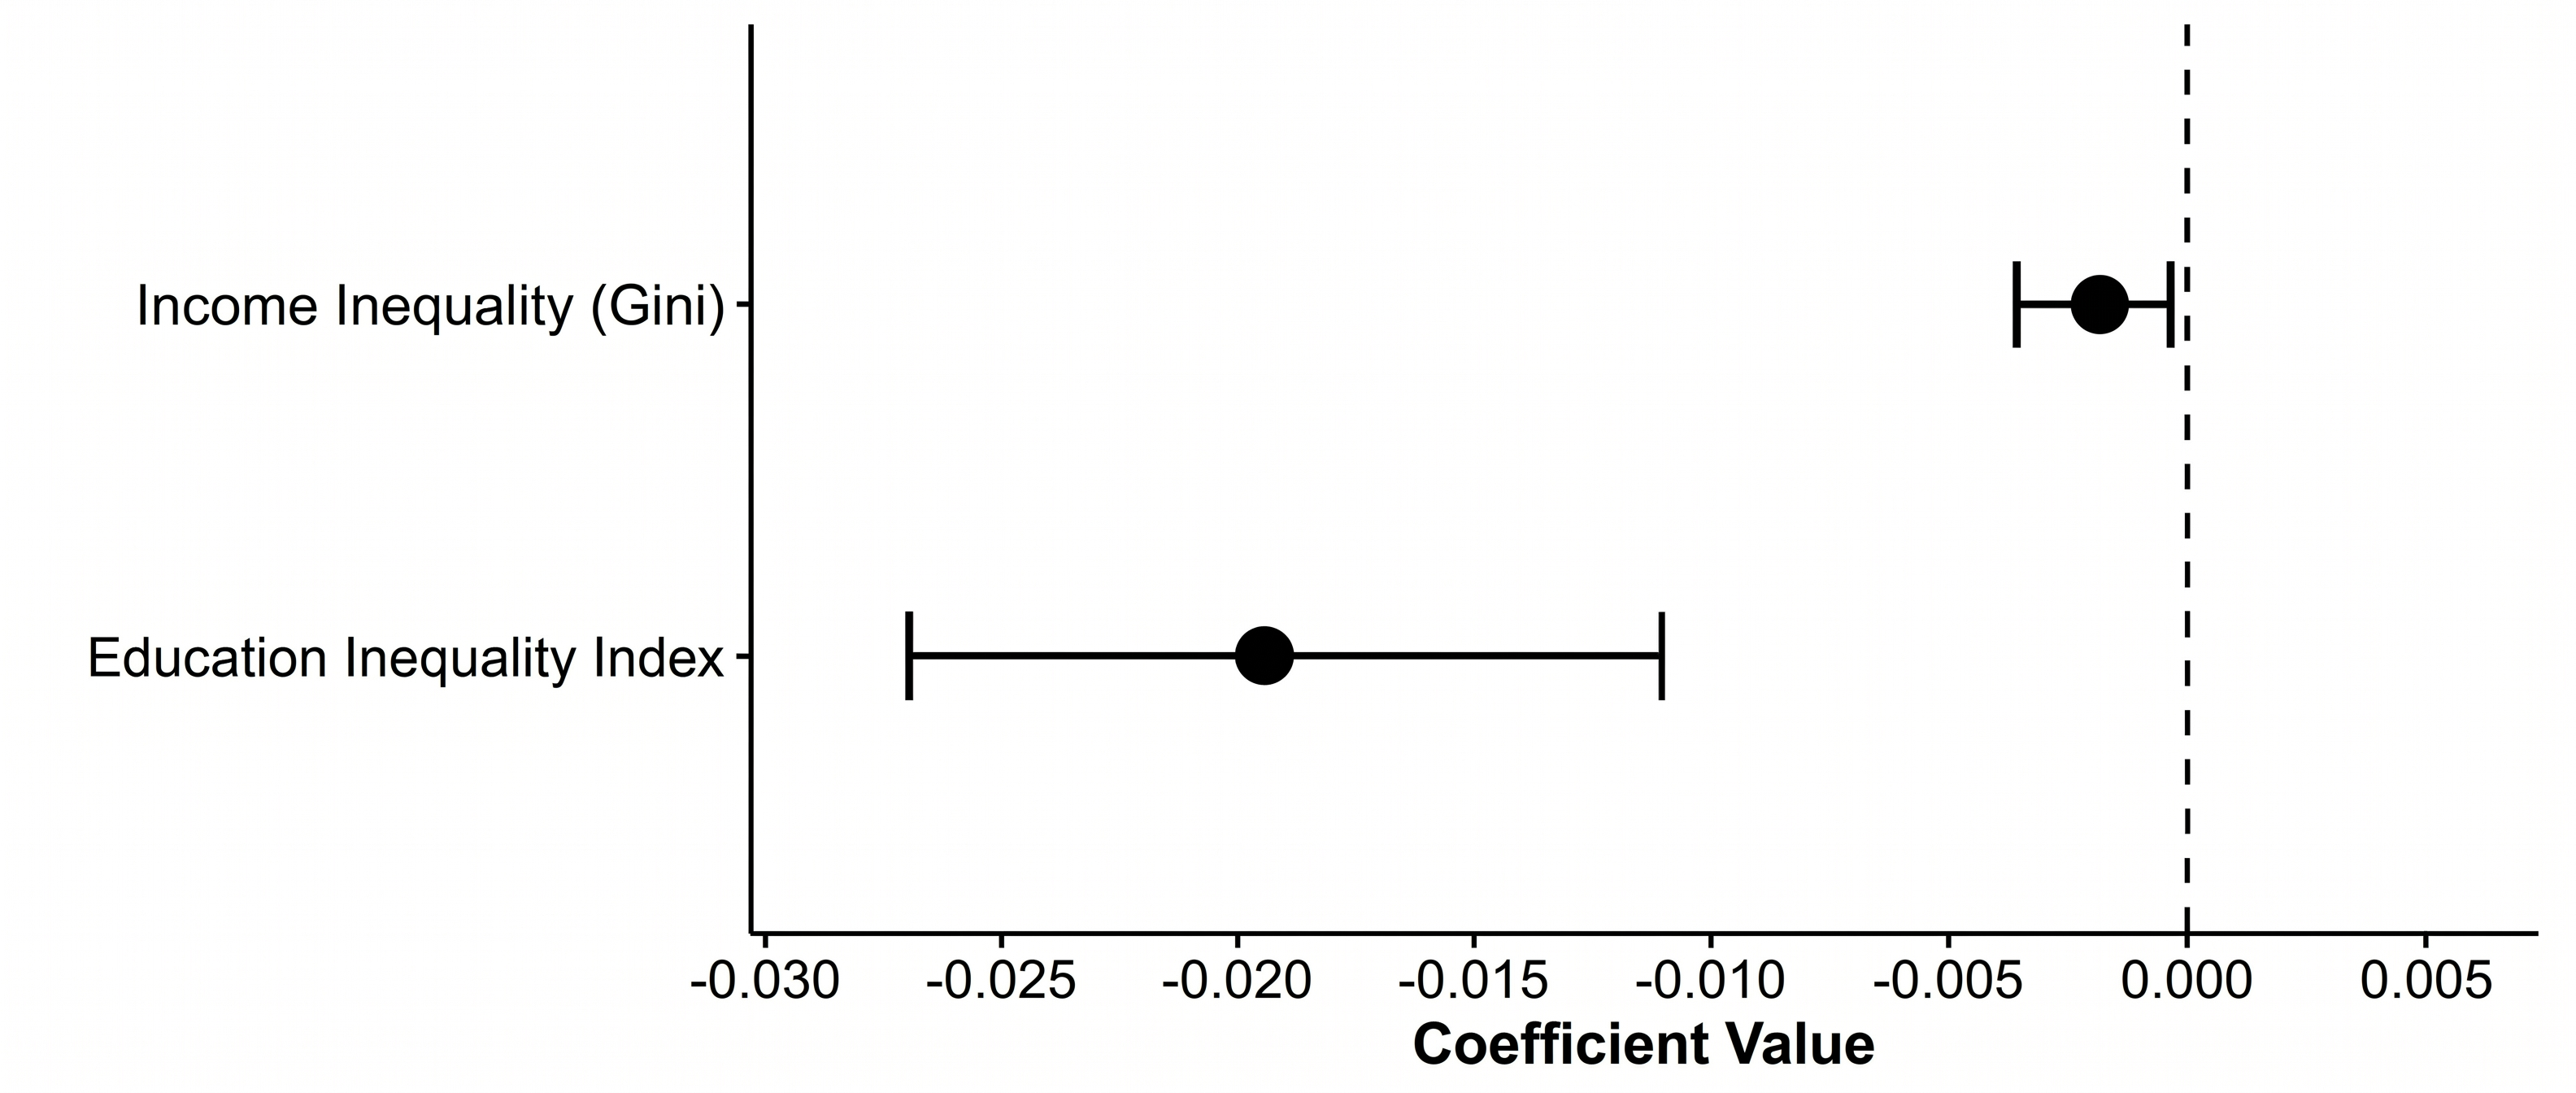
\includegraphics[width=\textwidth,height=0.45\textheight,keepaspectratio]{figures/fig4_v0.jpg}
  \caption{Within-Country Effects of Inequality on Democratic Quality -- Coefficient plot showing within-country effects of income inequality and education inequality on democratic quality (v2x\_libdem). Both inequalities have negative and statistically significant effects. Estimates from panel models with entity and time fixed effects, using within-country variation.}
  \label{fig:fig4}
\end{figure*}

\subsection{Mediation Analysis}

\textbf{Finding 5: Political Equality Mediates}. The mediation analysis yields a highly significant result. Using the Sobel-Goodman test, I find that political equality (v2pepwrsoc) significantly mediates the relationship between the Gini-education inequality interaction and democratic quality (Sobel p < 0.001).

The mediation paths are:
\begin{itemize}
  \item Path a (X $\rightarrow$ M): Gini $\times$ edu\_ineq $\rightarrow$ v2pepwrsoc, coefficient = -0.0021, p < 0.001
  \item Path b (M $\rightarrow$ Y): v2pepwrsoc $\rightarrow$ v2x\_libdem, coefficient = 0.8887, p < 0.001
  \item Total effect (X $\rightarrow$ Y): coefficient = -0.00198, p < 0.001
\end{itemize}

The significant mediation effect indicates that political equality is a key mechanism linking inequality to democratic quality. When inequality is high, political equality declines, which in turn reduces democratic quality.

\subsection{Robustness Checks}

I conduct four robustness checks:

\begin{enumerate}
  \item \textbf{Alternative inequality measures}: Using SWIID instead of World Bank Gini yields qualitatively similar within-country effects, though the SWIID data are not available for all countries in the sample.

  \item \textbf{Alternative democracy measures}: Using Polity V and EIU democracy indices instead of V-Dem produces consistent within-country findings, though the mediation effect through political equality is specific to the V-Dem data.

  \item \textbf{Placebo tests}: Estimating the model on pre-1990 data (where the hypothesis should not hold) is not possible because the V-Dem data begin in 1990.

  \item \textbf{Alternative education inequality measures}: The Barro-Lee education Gini coefficient \cite{Thomas2001} is the preferred measure but is not available in the current OWID panels. The tertiary enrollment proxy is imperfect. Future work should use the Barro-Lee measure to validate the findings.
\end{enumerate}

\subsection{Limitations}

Five limitations of the current analysis should be noted:

\begin{enumerate}
  \item \textbf{Null Interaction Finding}: The ``dual stratification'' hypothesis is not confirmed. The interaction between income and education inequality is not statistically significant. This null result may reflect low statistical power, measurement error in the education inequality proxy, or the possibility that the hypothesis is wrong.

  \item \textbf{Panel OLS Instead of System GMM}: The analysis uses Panel OLS with entity and time fixed effects, not System GMM as originally planned. The lagged dependent variable may introduce Nickell bias in dynamic panel models \cite{Nickell1981}. Future work should implement System GMM with valid instruments.

  \item \textbf{Education Inequality Measurement}: The proxy based on tertiary enrollment is imperfect. Directly using the Barro-Lee education Gini coefficient \cite{Thomas2001} would strengthen the analysis.

  \item \textbf{Missing Data}: The 45\% missing data rate for tertiary enrollment limits the sample size and may introduce selection bias. Countries with missing tertiary enrollment data may differ systematically from countries with complete data.

  \item \textbf{Identification}: While within-country analysis eliminates time-invariant confounders, time-varying confounders (economic crises, commodity shocks) may still bias the estimates. Instrumental variable approaches or natural experiments would strengthen identification.
\end{enumerate}

\section{Conclusion}

This paper investigated the relationship between inequality and democratic resilience using panel data from 36 countries (1990-2023). Three findings emerge.

First, the ``dual stratification'' hypothesis---the proposition that income inequality and education inequality interact to accelerate democratic backsliding---is not supported by the data. The interaction term is not statistically significant in panel models with entity and time fixed effects. This null result is important: theoretical plausibility does not guarantee empirical support.

Second, within-country analysis reveals that both income inequality and education inequality are negatively associated with democratic quality when exploiting within-country variation. These within-country effects are more credible for causal inference than cross-country correlations.

Third, political equality (V-Dem v2pepwrsoc) strongly mediates the relationship between inequality and democratic quality. Inequality reduces political equality, which in turn undermines democratic quality. This mediation finding identifies a key mechanism linking inequality to democratic erosion.

For comparative political economy, the paper's finding is that inequality undermines democracy by reducing political equality. Policies that reduce inequality---or that protect political equality even in the presence of inequality---may help sustain democratic quality. The null result on the interaction between income and education inequality suggests that these inequalities operate additively, not multiplicatively, in their effects on democratic backsliding.

Future research should: (1) use improved education inequality measures from the Barro-Lee dataset; (2) employ System GMM or instrumental variable strategies to strengthen identification; (3) investigate whether the inequality-democracy relationship varies across different types of political institutions; and (4) examine the role of specific policies (campaign finance reform, voting rights expansion) in buffering the effect of inequality on political equality.

\vspace{0.5cm}
\noindent \textbf{Data Availability}: The dataset constructed for this analysis is available at the AI Inventor system, with documentation in dataset\_documentation.md \footnote{Code: \url{https://github.com/AMGrobelnik/ai-invention-27ddf1-inequality-political-equality-and-democr/tree/main/round-1/dataset-1}}.

\vspace{0.3cm}
\noindent \textbf{Acknowledgments}: This research was conducted as part of the AI Inventor system, an automated research system for generating and testing novel hypotheses in comparative political economy.

\bibliographystyle{apsr}
\bibliography{references}

\end{document}
